\documentclass{article}
\usepackage[utf8]{inputenc}
\usepackage[polish]{babel}
\usepackage{polski}
\usepackage{enumerate}
\usepackage{natbib}
\usepackage{graphicx}
\usepackage{geometry}
\usepackage{float}

\newgeometry{tmargin=2.3cm, bmargin=2.5cm, lmargin=2.5cm, rmargin=2.5cm}

\makeatletter
\newcommand{\linia}{\rule{\linewidth}{0.4mm}}
\renewcommand{\maketitle}{\begin{titlepage}
    \vspace*{1cm}
    \begin{center}
    Politechnika Wrocławska\\
    AiR ARR\\
 Projekt zespołowy
    \end{center}
      \vspace{3cm}
    \begin{center}

     \LARGE \textsc {\@title}
         \end{center}
     \vspace{1cm}

    \begin{center}
    \textit{ Autorzy:}\\
   \textit{\@author}
     \end{center}
      \vspace{1cm}

     \begin{center}

    Prowadzący:
  dr inż. Krzysztof Arent
    \end{center}

    \vspace*{\stretch{6}}
    \begin{center}
    \@date
    \end{center}
  \end{titlepage}
}
\makeatother
\author{Beata Berajter\\
Dawid Brząkała\\
Dorota Gidel\\
Katarzyna Wądrzyk\\
Ada Weiss\\
Małgorzata Witka-Jeżewska\\
 }
\title{SensGlove}

\begin{document}

\maketitle
\newpage
\tableofcontents
\newpage



\section{Kryteria ewaluacji}
Komponenty powinny działać każde z osobna oraz współdziałać jako kompletne stanowisko do pobierania sygnałów i biosygnałów. Użytkownik powinien mieć możliwość wykonywania ruchów w obrębie przynajmniej jednego metra od stanowiska. Rękawiczka pomiarowa powinna mieć umieszczone czujniki w taki sposób, aby nie ograniczała ruchów ani tym bardziej nie krępowała ich. Pomiary przesyłane mają być w czasie rzeczywistym, a ich podgląd zapewnić ma program wizualizujący je.
\begin{enumerate}
	\item Założenie rękawiczki.
	\item Poruszanie palcami.
	\item Obserowanie przebiegów pomiarów.
	\item Rozpoczęcie pomiaru.
	\item Zapis pomiaru.
	\item Sprawdzenie katalogu, w którym dokonano zapisu.
\end{enumerate}
%%%%%%%%%%%%%%%%%%%%%%%%%
% Ogólnie:
% zrealizowane części projektu
% sposób ich zrealizowania
% niezrealizowane
% dlaczego nie
%
%
%
% Pozmieniałam tytuły dla punktu 2.1, prosze zrobić coś w tym właśnie stylu, chyba że macie lepsze propozycje - można tak jak w punkcie 2.4 robić
%
%
% UWAGA! Tekst specyfkacji zostawiam po to, zebyscie nei musieli szukać! Należy go usunać albo chociaż zmienić na swoje potrzeby
%%%%%%%%%%%%%%%%%%%%%%%%%
\section{Przebieg prac dla poszczególnych komponentów}
\subsection{Rękawiczka sensoryczna}
Osoby przydzielone do zadania: Dorota Gidel, Katarzyna Wądrzyk.
\subsubsection{Wykonanie rękawiczki}

Na rękawiczce wykonanej z poliestru przymocowano 10 czujników nasicku oraz 5 czujników ugięcia. Umiejscowienie czujników zotsało przedstawione na rysunku \ref{rys:czujniki_numeracja}.\\
\begin{figure}[H]
    \centering
    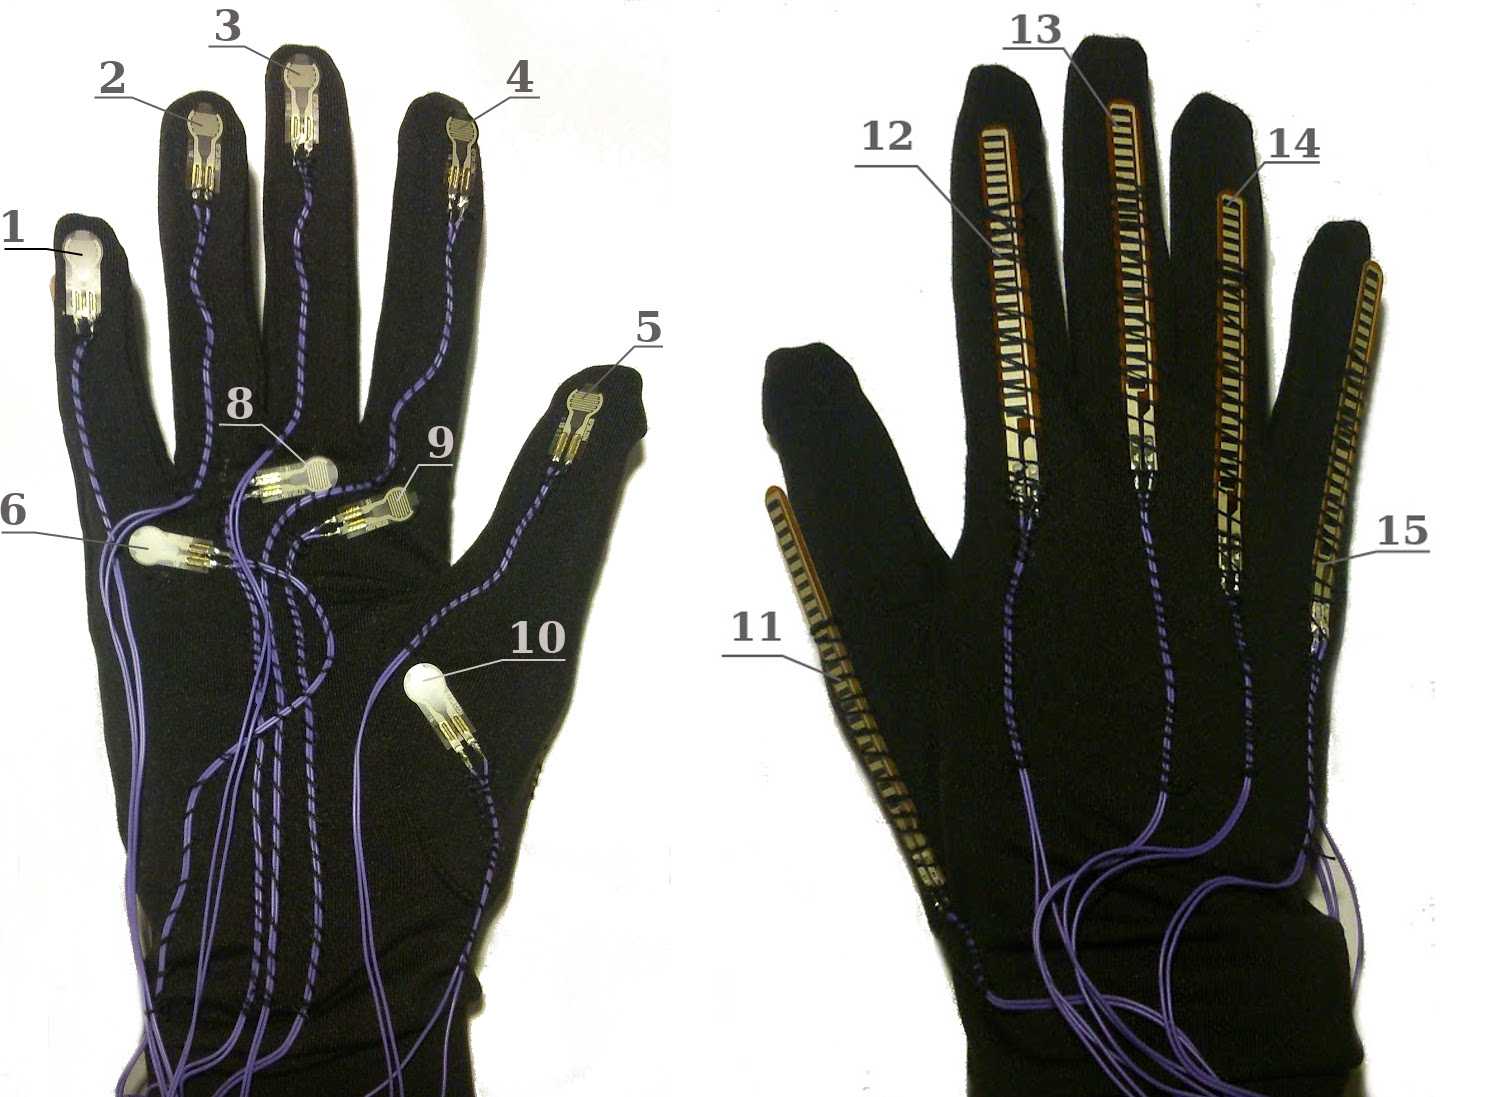
\includegraphics[width=14cm]{rekawiczka_umiejscowienie.jpg}
    \caption{Umiejscowienie i numeracja czujników na rękawiczce}
    \label{rys:czujniki_numeracja}
\end{figure}
Proces wykonania rękawiczki polegał na przylutowaniu przewodów do czujników, następnie przyklejeniu punktowo klejem czujników w odpowiednich miejscach na rękawiczce oraz przyszycie przewodów do rękawiczki, w przypadku czujników zgięcia przyszyto również część czujnika by mógł się poruszać. \\
Przyszycie przewodów pozwala na zachowanie porządku i sprzyja ruchom osoby używającej rękawiczkę a przytwierdzenie klejem zapewnia trwałość. W celu zapobiegania uszkodzenia czujników (przede wszystkim haczeniu) uszyte zostały ''kapturki'' na palce. Dzięki nim sensory nacisku jak i także ugięcia są zabezpieczone przed uszkodzeniami.\\
Na końcach przewodów odprowadzających sygnały z czujników zamontowane zostały żeńskie końce, które umożliwiają proste podłączenie ich do płytki wzmacniającej. Przymocowane czujniki numerowane są w kolejności przedstawioej na rysunku \ref{rys:czujniki_numeracja}.

\subsubsection{Wprowadzone zmiany}
Planowowane było kupienie rękawiczki w rozmiarze S, ze względu na skład grupy, jednakże ostatecznie wybrano rozmiar M. Rękawiczka nadal dobrze dopasowuje się na dłoniach małych ale dodatkowo może z niej korzystać większe grono osób. Dzięki czemu do tworzenia bazy danych nie będzie potrzeby specjalnie wybierania i szukania osób o danym rozmiarze dłoni.\\
Zaletą większego rozmiaru jest też większa powierzchnia do mocowania czujników. Dużo łatwiej jest rozmieścić wszystkie sensory, po ich przymocowaniu nie ograniczają one ruchów w tak dużym stopniu jakby miało to miejsce przy rękawiczce o rozmiarze S.\\
Ze względu uszkodzenia się czujników, rękawiczka posiada 9 czujników nacisku. Jak widać na zdjęciu \ref{rys:czujniki_numeracja} czujnik 7 został pominięty, a czujnik 8 lekko przesunięty w lewą stronę by to zrekompensować. Jednakże dalej isnieje możliwość przymocowania brakującego czujnika 7.

\subsubsection{Kryteria ewaluacji}
Jeden czujnik z wewnętrznej części dłoni został uszkodzony. Kilka czujników nacisku zostało odczepionych, ponieważ zostały przyklejone za nisko na placu, co powodowało złe odczyty przy chwytaniu przedmiotów. \\
Rękawiczka spełnia następujące kryteria:\\
\begin{enumerate}
  \item Rękawiczka założona na rękę pozwala na możliwie swobodne poruszanie palcami.
  \item Rezystancja czujników nacisku wraz ze wzrostem siły maleje, a wraz ze stopniem zgięcia rezystancja czujników zgięcia rośnie.
	\item Przy chwytaniu przedmiotów czujniki ugięcia działają sprawnie.
	\item Podczas wykonywania ruchów czujniki oraz przewody nie haczą się o nic dzięki dołączonym kapturkom.
	\item Po nałożeniu kapturków sensory na wewnętrznej części dłoni sprawnie odczytują siłę nacisku.
	\item Sygnały z czujników prowadzone przez przewody mogą być bezpośrednio podłączone do styków na wzmacniaczu dzięki ich żeńskim końcówkom.
\end{enumerate}
Pomyślnie przeprowadzono próbę integracji rękawiczki z prototypem płytki wzmacniającej. Miernikiem mierzono napięcie, które jak oczekiwano zmieniało odpowiednio swoją wartość. Sprawdzone zostały zarówno czujniki zgięcia jak i nacisku.

\subsection{Interfejs sprzętowy}

Osoby przydzielone do zadania: Beata Berajter i Dawid Brząkała. \\
%odniesc sie trzeba jakos do tych kryteriów, co juz jest zrobione, moze zdjecie pcb, 
\subsubsection{Schemat układu}
\begin{figure}[!h]
	\centering
	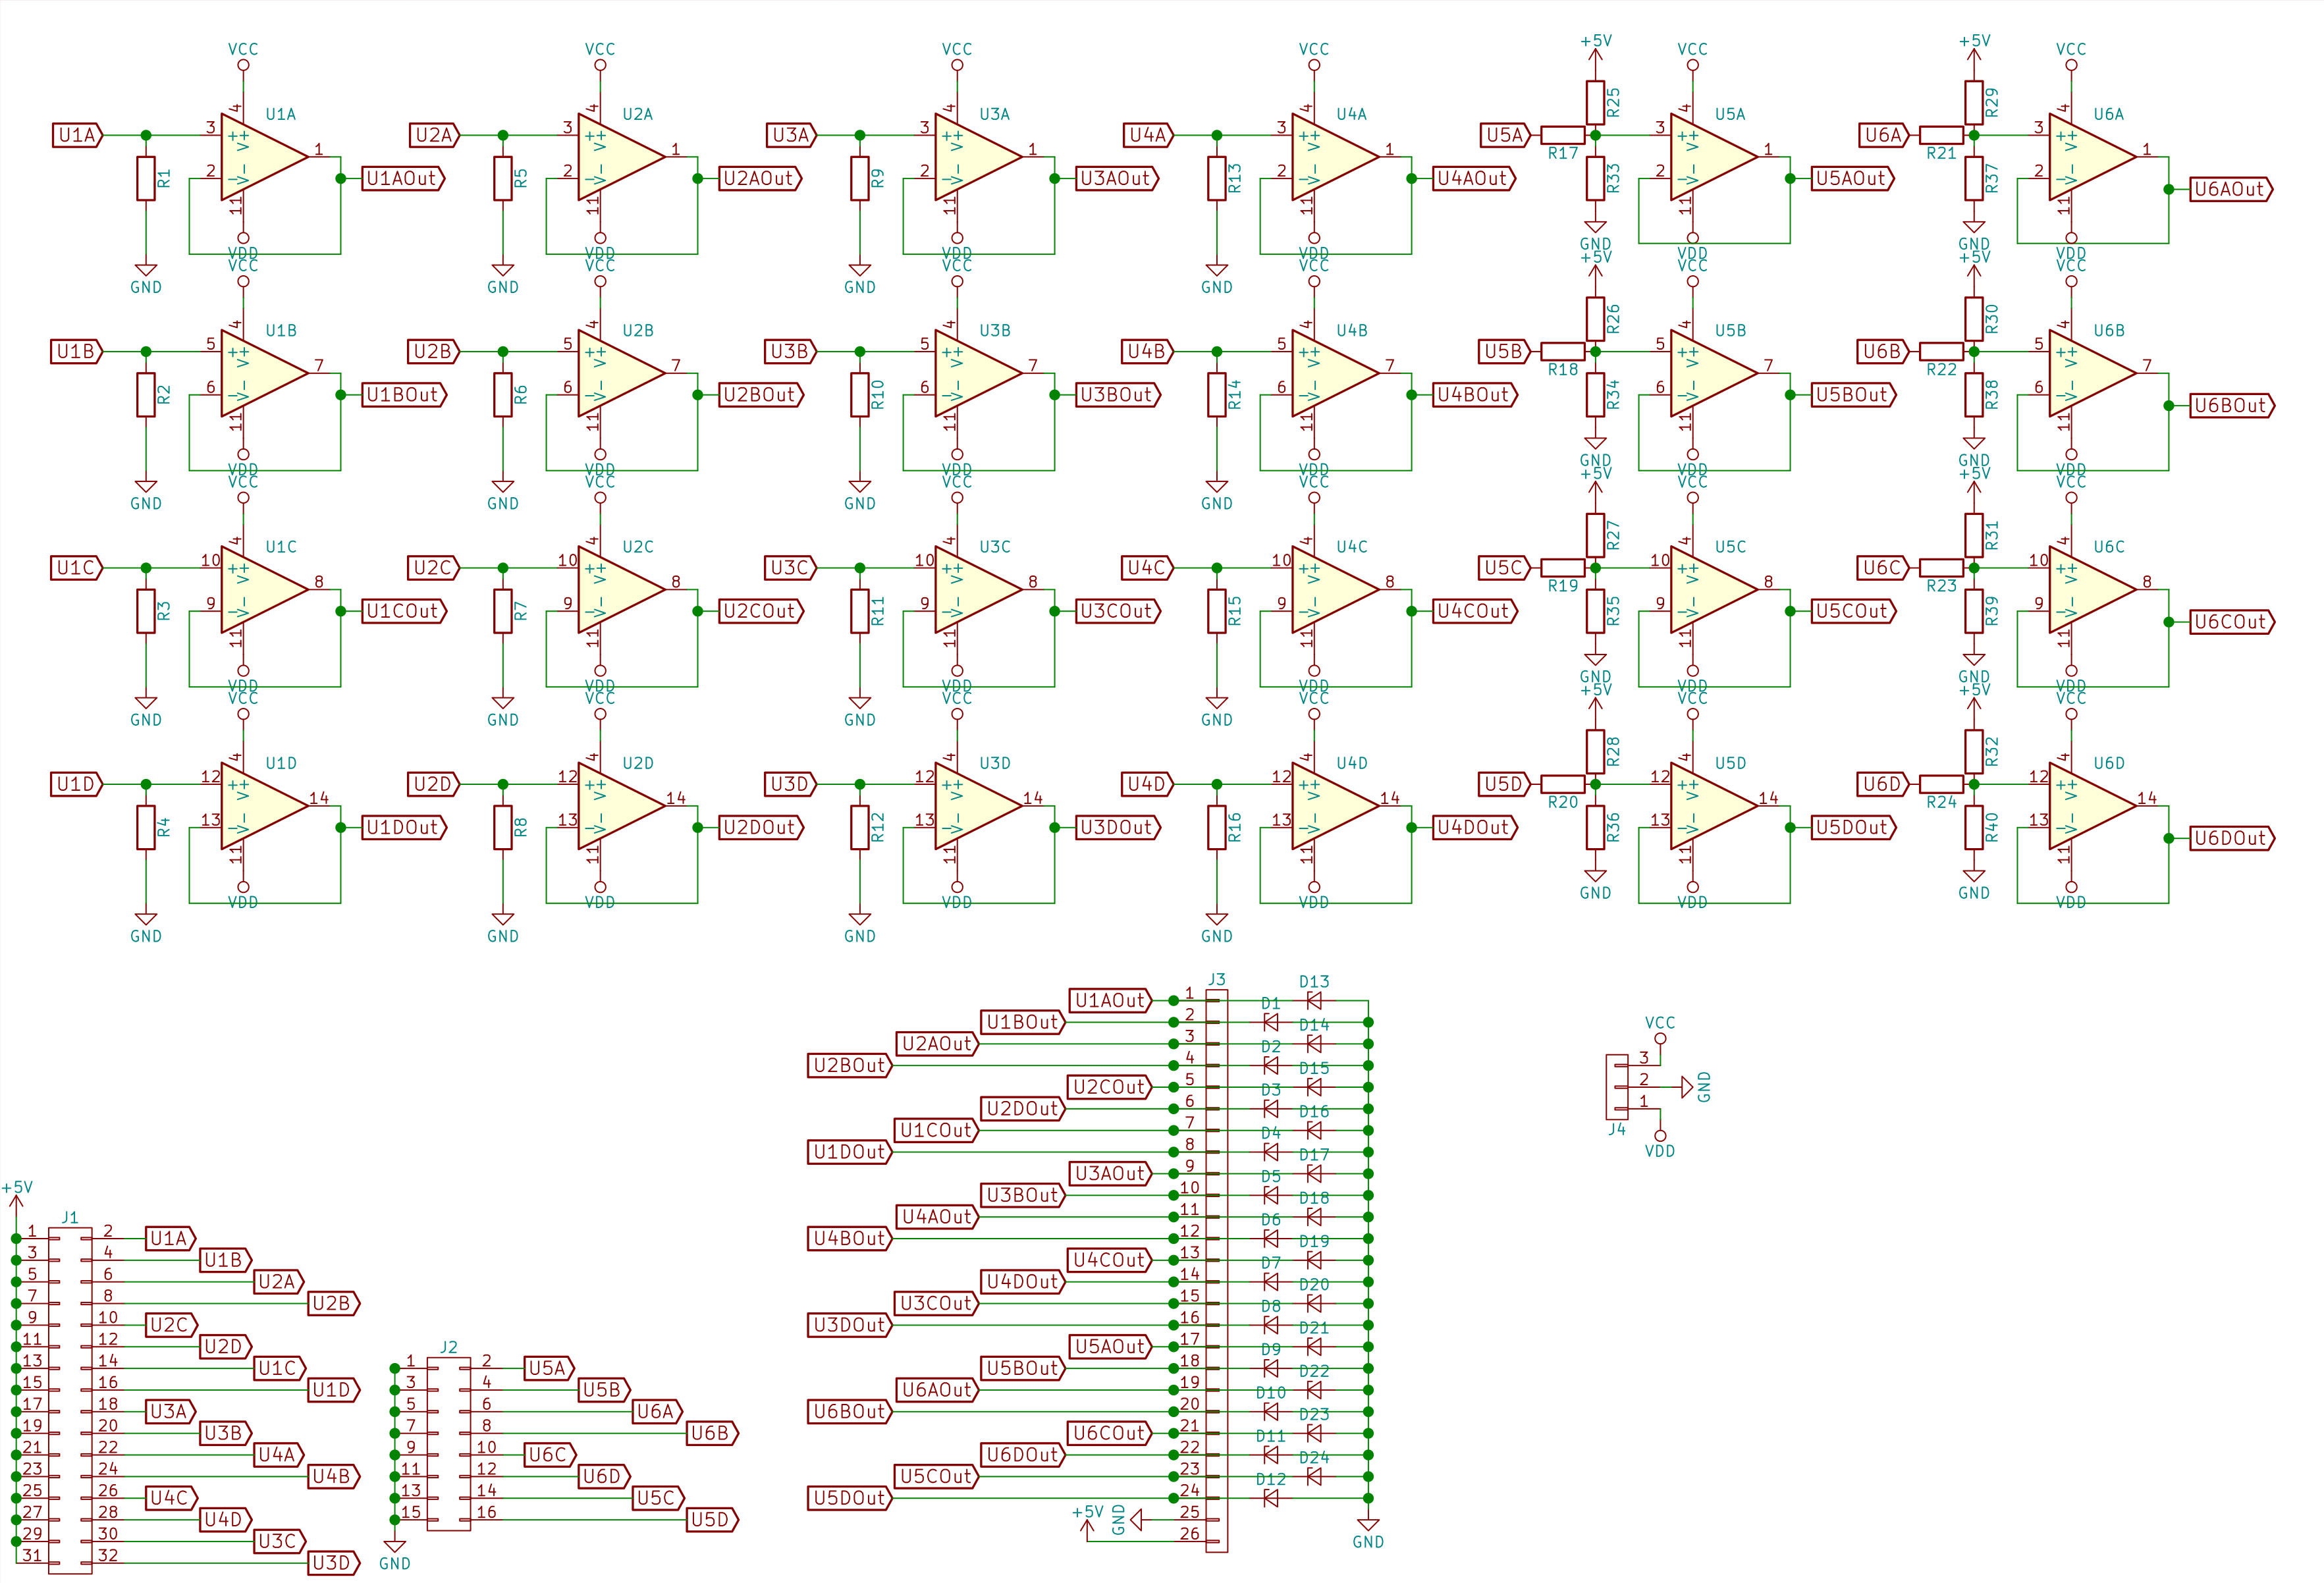
\includegraphics[width=15cm]{schemat.png}
	\caption{schemat układu}
	\label{rys:schemat_ukladu}
\end{figure}

Projekt płytki pcb i wyprowadzenie pinów układu przedstawiono na rysunku  \ref{rys:pcb}.

\begin{figure}[H]
	\centering
	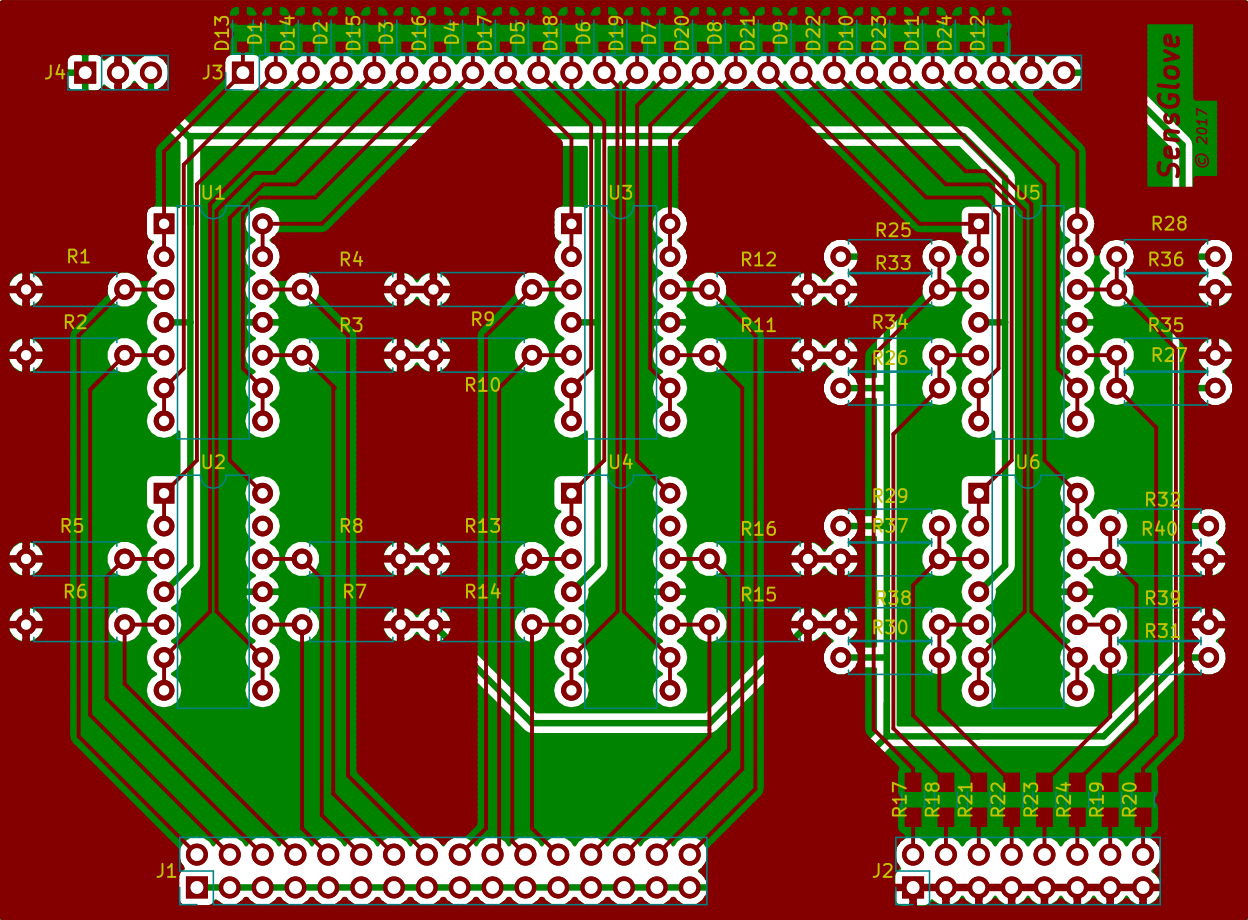
\includegraphics[width=12cm]{pcb.png}
	\caption{Schemat płytki pcb}
	\label{rys:pcb}
\end{figure}

\begin{figure}[H]
	\centering
	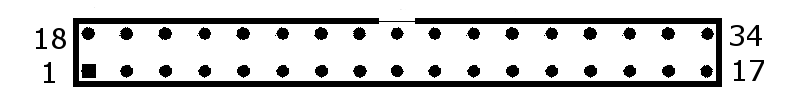
\includegraphics[width=9cm]{J1.png}
	\caption{J1 - pinout}
	\label{rys:J1 - pinout}
\end{figure}

\begin{table}[H]
	\centering
	\label{J1 - pinout}
	\begin{tabular}{ll}
	1 - 16		&	zasilanie czujników - +5v		\\
	17 - 27		&	złącza czujników nacisku 1 - 10		\\
	28 - 33		&	złącza czujników ugięcia 1 - 6		\\
	2, 34		&	NC					\\
\end{tabular}
\end{table}

\begin{figure}[H]
	\centering
	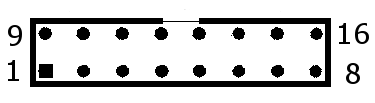
\includegraphics[width=9cm]{J2.png}
	\caption{J2 - pinout}
	\label{rys:J2 - pinout}
\end{figure}

\begin{table}[H]
	\centering
	\label{J2 - pinout}
	\begin{tabular}{ll}
	1 - 7		&	GND					\\
	8 - 16		&	złącza czujników biosygnałów 1 - 8	\\
\end{tabular}
\end{table}

\begin{figure}[H]
	\centering
	
\includegraphics[width=9cm]{J3.png}
	\caption{J3 - pinout}
	\label{rys:J3 - pinout}
\end{figure}

\begin{table}[H]
	\centering
	\label{J3 - pinout}
	\begin{tabular}{ll}
	1 - 10		&	sygnał czujników nacisku 1 - 10		\\
	11 - 16		&	sygnał czujników ugięcia 1 - 6		\\
	17 - 24		&	sygnał czujników biosygnałów 1 - 8	\\
	25		&	+5V					\\
	26		&	GND					\\
\end{tabular}
\end{table}

\begin{figure}[H]
	\centering
	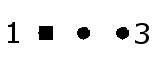
\includegraphics[width=9cm]{J4.png}
	\caption{J4 - pinout}
	\label{rys:J4 - pinout}
\end{figure}

\begin{table}[H]
	\centering
	\label{J4 - pinout}
	\begin{tabular}{ll}
	1 		&	-9V					\\
	2		&	GND					\\
	3		&	+9V					\\
\end{tabular}
\end{table}

\subsubsection{Lista elementów}
\begin{table}[H]
	\centering
	\label{Bill of materials}
\begin{tabular}{lll}
U1-U6		&	TLC084CN			&	THT	\\
R1-R10		&	10kOhm				&	THT	\\
R11-R16		&	33kOhm				&	THT	\\
R17-R24		&	3.3kOhm				&	SMD	\\
R25-R32		&	3.3kOhm				&	THT	\\
R33-R40		&	2.2kOhm				&	THT	\\
D1-D24		&	3.3V Zenera			&	SMD	\\
J1		&	IDC-34 żeńskie			&	THT	\\
J2		&	IDC-16 żeńskie			&	THT	\\
J3		&	listwa kołkowa 1x26 2.56mm	&	THT	\\
J4		&	listwa kołkowa 1x3 2.56mm	&	THT	\\
\end{tabular}
\end{table}

\subsubsection{Połączenie z płytką STM32F3Discovery}
\begin{table}[H]
	\centering
	\label{Bill of materials}
\begin{tabular}{ll}
J1		&	ST3M32Discovery	\\
1		&	PB12		\\
2		&	PB14		\\
3		&	PB15		\\
4		&	PD8		\\
5		&	PD9		\\
6		&	PD10		\\
7		&	PD11		\\
8		&	PD12		\\
9		&	PD13		\\
10		&	PD14		\\

11		&	PB0		\\
12		&	PB1		\\
13		&	PE7		\\
14		&	PE8		\\
15		&	PE9		\\
16		&	PE10		\\

17		&	PA0		\\
18		&	PA3		\\
19		&	PA2		\\
20		&	PF4		\\
21		&	PA4		\\
22		&	PA5		\\
23		&	PA6		\\
24		&	PA7		\\

25		&	GND		\\
26		&	5V		\\
\end{tabular}
\end{table}

\subsection{Kod programu}
\begin{verbatim}
//struktura danych do zapisu odczytu sygnałów
typedef union
{
	struct
	{
		uint16_t forceSensors[10];
		uint16_t flexSensors[6];
		uint16_t biosignals[8];
		uint16_t checksum;
	}measure;
	uint16_t measures[25];
} data_t;
data_t data;

...

//konfiguracja DMA
  HAL_ADC_Start_DMA(&hadc1, &data.measure.biosignals[0], 4);
  HAL_ADC_Start_DMA(&hadc2, &data.measure.biosignals[4], 4);
  HAL_ADC_Start_DMA(&hadc3, &data.measure.flexSensors[0], 6);
  HAL_ADC_Start_DMA(&hadc4, &data.measure.forceSensors[0], 10);

...

  data.measure.checksum = 0;
  for(int i = 0; i < 24; i++)
  {
    data.measure.checksum+=data.measures[i];
  }
  printf("X%4.4x%4.4x%4.4x%4.4x%4.4x%4.4x%4.4x%4.4x%4.4x%4.4x%4.4x%4.4x%4.4x%4.4x%4.4x%4.4x%4.
  4x%4.4x%4.4x%4.4x%4.4x%4.4x%4.4x%4.4x%4.4x\r\n",
	  data.measures[0], data.measures[1], data.measures[2], data.measures[3], data.measures[4],
	  data.measures[5], data.measures[6], data.measures[7], data.measures[8], data.measures[9],
	  data.measures[10], data.measures[11], data.measures[12], data.measures[13], data.measures[14],
	  data.measures[15], data.measures[16], data.measures[17], data.measures[18], data.measures[19],
	  data.measures[20], data.measures[21], data.measures[22], data.measures[23], data.measures[24]);
\end{verbatim}

\subsubsection{Kryteria ewaluacji}
Poprawność odczytu sygnałów przez układ wzmacniaczy sygnałów sprawdzono poprzez podłączenie potencjometrów w miejsce czujników i pomiar napięć na wyjściu. Sprawdzono również współpracę z rękawiczką. 
Poprawność odczytu sygnałów przez płytkę Discovery sprawdzono poprzez odczyt wartości zmiennych w pamięci mikrokontrolera przy użyciu programu STMStudio.
Poprawność samej transmisji sprawdzona została poprzez wysyłanie pomiarów przez kabel USB i porównywanie z wartościam w pamięci mikrokontrolera.\\
\\
Na obecnym etapie pracy zauważono błędne sygnały na 6, 9 i 14 złączu J3.\\
Należy również przeprowadzić weryfikację poprawności odczytu biosygnałów.

%%%%%%%%%%%%%%%%%%%%%%%%%
\subsection{Program do akwizycji danych}

Osoby przedzielone do zadania: Ada Weiss, Małgorzata Witka-Jeżewska
\subsection{Opis klas programu}
Dokładny opis klas i poszczególnych parametrów tworzony jest za pomocą programu Doxygen.
\begin{figure}[h!]
    \centering
    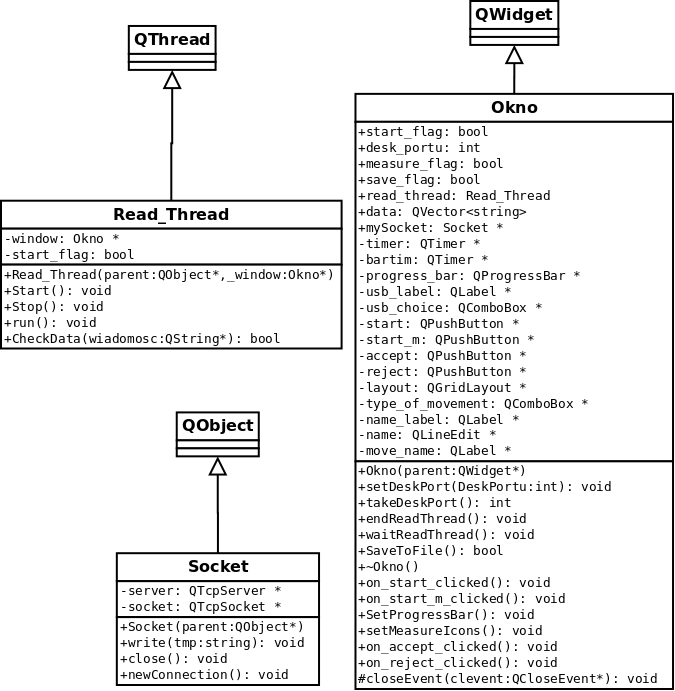
\includegraphics[scale=0.4]{autodia.png}
    \caption{Diagram klas programu}
    \label{rys:autodia}
\end{figure}

\begin{figure}[h!]
    \centering
    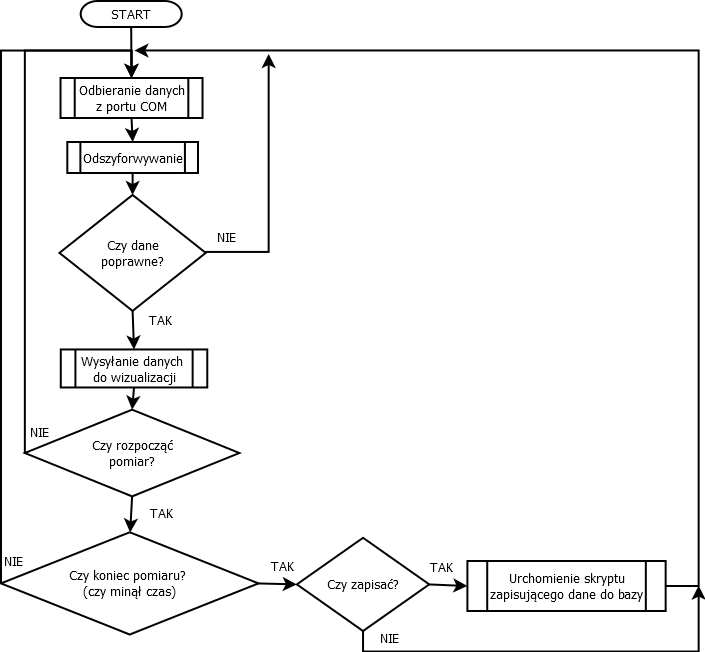
\includegraphics[scale=0.6]{programdia.png}
    \caption{Schemat ideowy działania programu}
    \label{rys:programdia}
\end{figure}

\subsubsection{Opis działania programu}

Interfejs graficzny programu został napisany z wykorzystaniem klas biblioteki Qt5 i został zaprezentowany na rys. \ref{rys:okno}. 
\begin{figure}[h!]
    \centering
    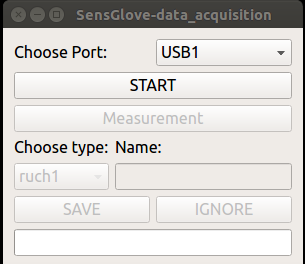
\includegraphics[scale=0.6]{okno.png}
    \caption{Okno główne programu}
    \label{rys:okno}
\end{figure}

Zasada działania została przedstawiona na rys. \ref{rys:programdia}. 
Pierwszym krokiem jest wybór portu USB i wciśnięcie przycisku start, co uruchamia konfiguracje wybranego portu USB. W przypadku braku podłączonego urządzenia na danym porcie wyświetlany jest komunikat przedstawiony na rys. \ref{rys:oknousb}. Kliknięcie "Yes" umożliwia ponowny wybór, a "No" kończy pracę programu.\\
\begin{figure}[h!]
    \begin{center}
    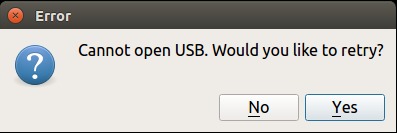
\includegraphics[scale=0.6]{oknousb.png}
    \caption{Komunikat o błędnym otwarciu USB.}
    \label{rys:oknousb}
    \end{center}
\end{figure}
Dane są odczytywane z poru USB w oddzielnym wątku Read\_thread, dziedziczącego po QThread. Zapewnia to odpowiednio szybką pracę programu. W tym samym wątku sprawdzana jest poprawność otrzymanej wiadomości (obliczanie sumy kontrolnej, sprawdzanie dlugości ciągu znaków) oraz wysyłanie danych do Socketu, który również został zaprogramowany z wykorzystaniem bibliotek Qt5 (klasa Socket).

W przypadku aktywowania przycisku "Measurment" aktywowany jest timer (na 2s) i dane te są zapisywane w wektorze 2000x23, z którego to jest możliwość zapisu danych do pliku w przypadku akceptacji pomiaru po jego ukończeniu. Widok okna w trakcie pomiaru przedstawia \ref{rys:oknopomiar}.
\begin{figure}[h!]
    \centering
    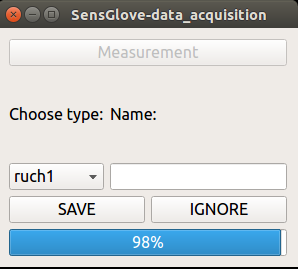
\includegraphics[scale=0.6]{oknopomiar.png}
    \caption{Okno główne programu w trakcie pomiaru}
    \label{rys:oknopomiar}
\end{figure}

Akceptacja pomiaru wymaga również podania imienia użytkownika oraz wyboru ruchu który jest wykonywany. Program wywołuje po zapisie do pliku skrypt który umieszcza plik w bazie danych.

Można również dany pomiar zignorować, np. w przypadku stwierdzenia, że został on błędnie wykonany.

\subsubsection{Format danych}
Ramka danych:
\begin{itemize}
    \item znak X,
    \item 23 sygnały z czujników w postaci 4 znaków w systemie szesnastkowym,
    \item suma kontrolna w postaci dwóch znaków w systemie szesnastkowym,
    \item znak końca linii \textbackslash r \textbackslash n;
\end{itemize}

\subsubsection{Raport z ewaluacji}
Do symulowania danych wejściowych zaprogramowano płytkę STM32F476G Discovery tak, aby nadawała przykładowe dane w ustalonym przez nas formacie poprzez odpowiednią konfigurację USB. \\
Do sprawdzenia poprawności przesyłu danych wykorzystany został program telnet. Dane nadawane są na porcie 2666 (planowane jest dodanie możliwości wyboru portu, na którym dane będą nadawane). Przesył danych był poprawny. \\
Dane były również wysyłane do programu do wizualizacji rękawiczki poprzez wspólny router Wi-Fi do drugiego komputera. Przesyłanie odbywało się bez zarzutów.

%%%%%%%%%%%%%%%%%%%%%%%%%
\subsection{Baza danych}
Osoby przydzielone do zadania: Beata Berajter, Dorota Gidel.

\subsubsection{Wprowadzone zmiany}
Zdecydowano się na zmianę struktury bazy danych. Zamiast umieszczania trzech osobnych plików zawierających dane odpowiednio z czujników nacisku, zgięcia i elektrod, tworzony będzie tylko jeden plik zawierający wszystkie te dane w takiej kolejności. Plik taki zawierać będzie 2000 linii i 23 kolumny odczytów. Dodatkowo, nazwa pliku nie będzie zawierać daty gdyż można ją uzyskać z daty tworzenia pliku. Nowy schemat struktury bazy danych przedstawiono na rysunku \ref{rys:baza_danych}.
\begin{figure}[H]
    \centering
    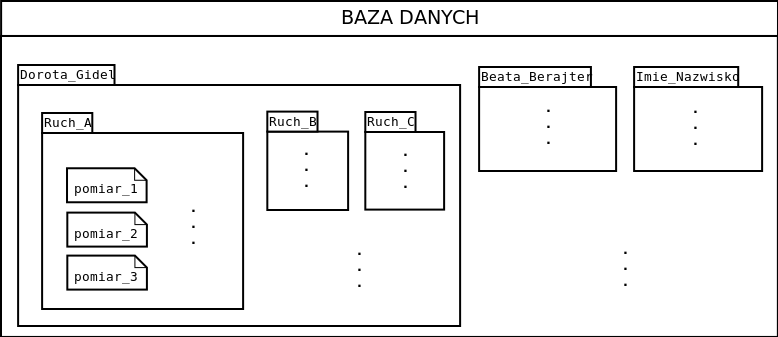
\includegraphics[width=\textwidth]{baza_danych.png}
    \caption{Schemat struktury bazy danych}
    \label{rys:baza_danych}
\end{figure}

\subsubsection{Opis działania skryptu}
Stworzony skrypt do umieszczania w odpowiednim miejscu plików z odczytami napisany jest w powłoce bash. Przykładowe wywołanie skryptu wgląda następująco:\\

\texttt{\$ bash przeniesPlik sciezka/do/pliku/z/danymi Imie NazwaRuchu}\\ \\
Skrypt przenosi podany plik (\texttt{sciezka/do/plik/z/danymi}) do głownego folderu bazy danych który zdefiniowany jest jako katalog o nazwie ''baza\_danych'' w katalogu domowym. Dzięki podanym argumentom umieszcza plik w odpowiednim miejscu. Numeracja pliku po kolei jest zapewniona przez prowadzenie spisu w osobnym pliku tekstowym należącym do bazy danych. Dla bezpieczeństwa sprawdzane jest też czy w wywołaniu skryptu została podana wystarczająca liczba argumentów.

\subsubsection{Kryteria ewaluacji}
Do sprawdzania poprawności działania bazy danych wywołano skrypt z przykładowymi argumentami. Otrzymano oczekiwane efekty, tj. utworzenie w odpowiednim miejscu w strukturze katalogów pliku o pożądanej nazwie (indeksie zwiększającym swoją wartość przy kolejnych przenoszeniach pliku do tego samego katalogu).

%%%%%%%%%%%%%%%%%%%%%%%%%
\subsection{Wizualizacja danych}
Osoby przydzielone do zadania: Dorota Gidel, Katarzyna Wądrzyk.

\subsubsection{Ogólny diagram klas}
Na rysunku \ref{rys:diagram_ogolny} zaprezentowano ogólny diagram klas w programie wizualizującym dane z czujników.
\begin{figure}[H]
    \centering
    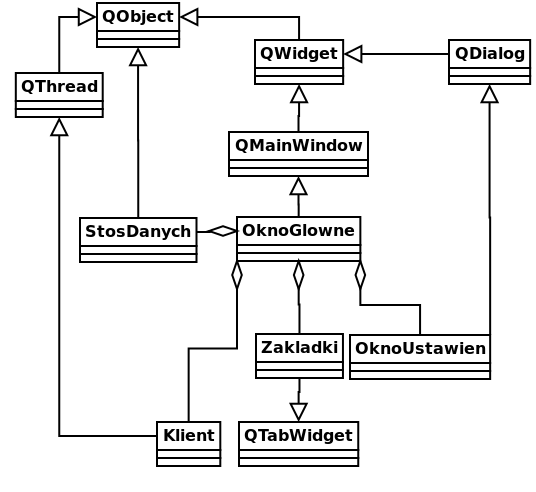
\includegraphics[width=11cm]{diagram_ogolny.png}
    \caption{Ogólny diagram klas - wizualizacja}
    \label{rys:diagram_ogolny}
\end{figure}

\subsubsection{Diagram klas zakładek}
Na obrazku \ref{rys:diagram_klas} zaprezentowano ogólny diagram klas zakładek zawierających wykresy i prezentacje odpowiednio z czujników nacisku oraz zgięcia.
\begin{figure}[H]
    \centering
    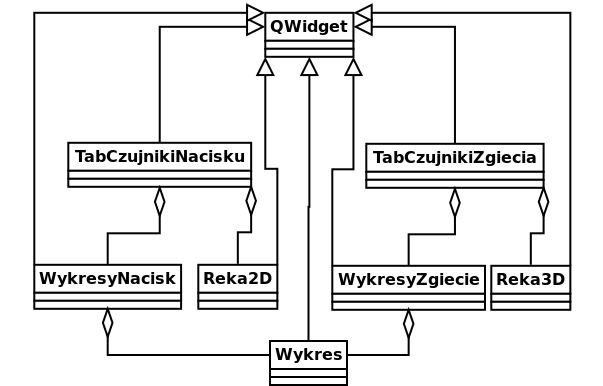
\includegraphics[width=11cm]{diagram_klas.png}
    \caption{Diagram klas zakładek - wizualizacja}
    \label{rys:diagram_klas}
\end{figure}

\subsubsection{Interfejs użytkownika}
Użytkownik ma możliwość połączenia się z portem nadającym dane przez przyciśnięcie przycisku ''Ustal nowe połączenie''. W trakcie odbierania danych istnieje możliwość zatrzymania wykresów i wizualizacji dłoni w danym momencie poprzez przyciśnięcie przycisku ''Stop''. W lewym górnym rogu użytkownik ma dostęp do ustwień w których obecnie może zmienić zakres czasu prezentowanego na wykresach. Domyślnie wartość ta wynosi 30 s.\\
Rysunek \ref{rys:zakladka1} przedstawia pierwszą zakładkę aplikacji wizualizującej dane - czujniki nacisku. Po lewej stronie umieszczone są wykresy. Pierwszy największy wykres, można zmieniać przyciskając odpowiednio wykres który chcemy najbardziej śledzić. Wybrany wykres zaznaczony jest przez kolorową obwódkę. Po prawej stronie znajduje się widget zawierający ręke 2D prezentującą przez kolory odczytywane w danym momencie wartości napięcia.
\begin{figure}[H]
    \centering
    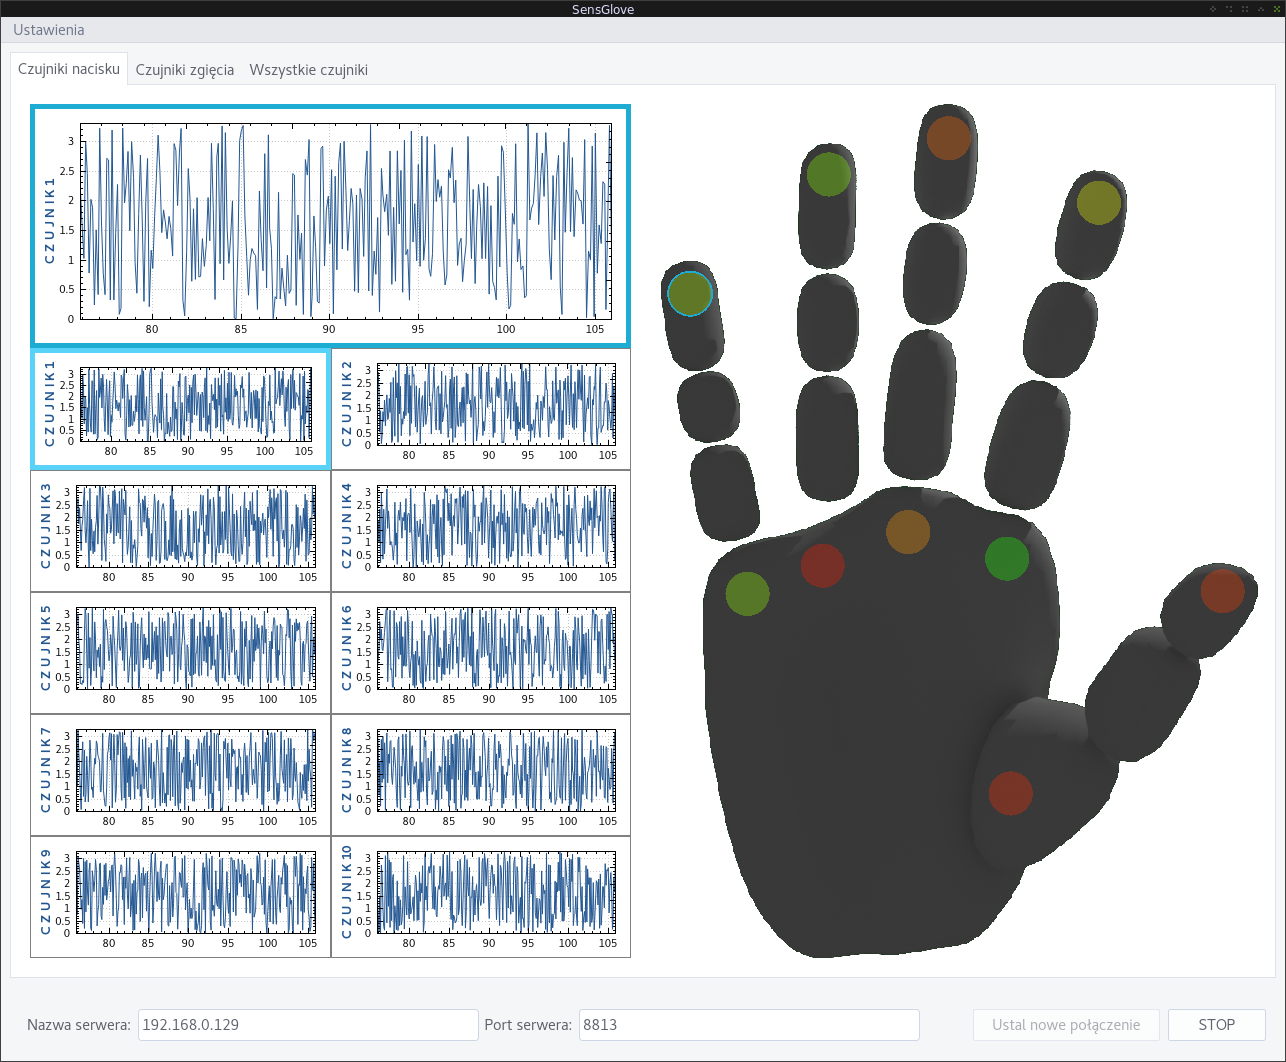
\includegraphics[width=18cm]{zakladka1.png}
    \caption{Diagram klas zakładek - wizualizacja}
    \label{rys:zakladka1}
\end{figure}
Rysunek \ref{rys:zakladka2} przedstawia drugą zakładkę aplikacji wizualizującej dane - czujniki zgięcia. Po lewej stronie tak samo jak poprzednio znajdują się wykresy odczytywanego napięcia. Po prawej stronie znajduje się widget zawierający ręke 3D której palce zginają się odpowiednio do otrzymywanych wartości z czujników.
\begin{figure}[H]
    \centering
    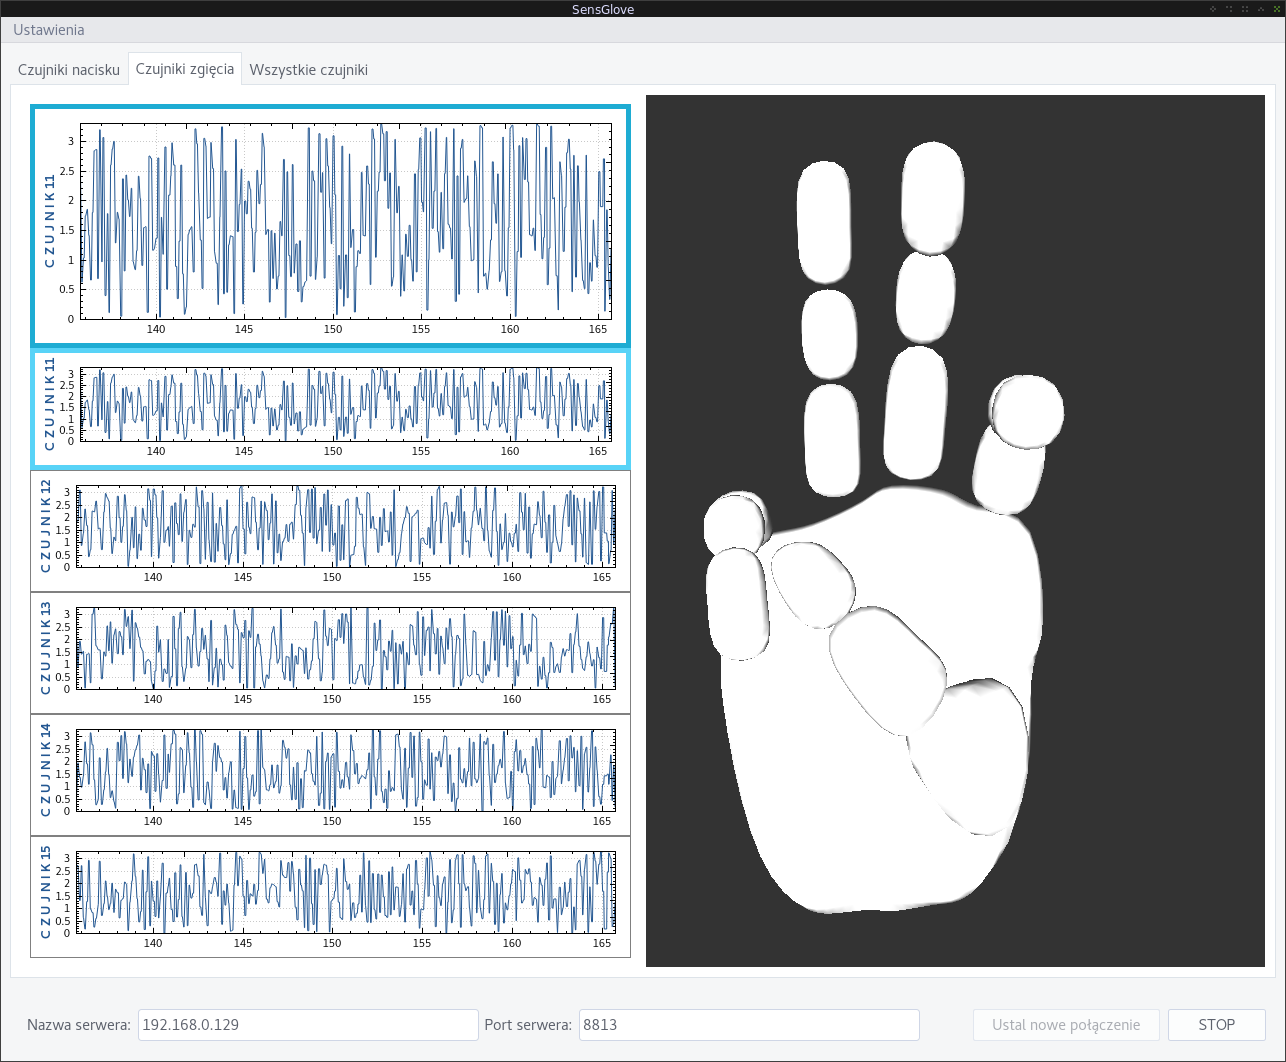
\includegraphics[width=18cm]{zakladka2.png}
    \caption{Diagram klas zakładek - wizualizacja}
    \label{rys:zakladka2}
\end{figure}

\subsubsection{Kryteria ewaluacji}
Do testowania poprawności działania aplikacji napisano dodatkowy program mający udawać serwer nadający dane. Program ten napisany jest w C. Dane które generuje są randomowe, a port, częstotliwość i ilość wysyłanych wiadomości podaje się jako jego argumenty.\\
Aplikacja odbiera pomyślnie zasymulowane dane z dodatkowego programu oraz wizualizuje zinterpretowane pomiary na wykresach i modelach dłoni. Przeprowadzono też integrację tej aplikacja z aplikacją to akwizycji dancyh, która przebiegła pomyślnie.

\subsection{Ewaluacja końcowa projektu}
Po połączeniu wszytkich komponentów projektu przeprowadzono testy. Polegały one na wykonywaniu ruchów w rękawiczce sensorycznej i obserwowanie efektów w programie wizualizującym oraz sprawdzenie poprawnego zapisu pliku do bazy danych. Testy pokazały, że sygnały przeysłane są odbierane poprawnie, co pokazują zdjęcia i film umieszczony na stronie internetowej sensglove.happyrobotics.com w odpowiednich zakładkach.

\end{document}
